\documentclass[9pt,twocolumn,twoside,lineno]{pnas-new}
% Use the lineno option to display guide line numbers if required.

\usepackage{siunitx}
\usepackage{physics}

\templatetype{pnasresearcharticle} % Choose template 
% {pnasresearcharticle} = Template for a two-column research article
% {pnasmathematics} %= Template for a one-column mathematics article
% {pnasinvited} %= Template for a PNAS invited submission

\title{A multi-control climate policy process for a trusted decision maker}

% Use letters for affiliations, numbers to show equal authorship (if applicable) and to indicate the corresponding author
\author[a,b,1]{Henri F. Drake}
\author[a]{Ronald L. Rivest} 
\author[a]{Alan Edelman}
\author[a]{John Deutch}

\affil[a]{Massachusetts Institute of Technology, 77 Massachusetts Ave, Cambridge, MA 02139, USA}
\affil[b]{MIT-WHOI Joint Program in Oceanography/Applied Ocean Science \&
Engineering, Cambridge and Woods Hole, MA, 02139, USA}

% Please give the surname of the lead author for the running footer
\leadauthor{Drake} 

% Please add a significance statement to explain the relevance of your work
\significancestatement{Authors must submit a 120-word maximum statement about the significance of their research paper written at a level understandable to an undergraduate educated scientist outside their field of speciality. The primary goal of the significance statement is to explain the relevance of the work in broad context to a broad readership. The significance statement appears in the paper itself and is required for all research papers.}

% Please include corresponding author, author contribution and author declaration information
\authorcontributions{All authors contributing to the conception of the project, interpretation of the results, and writing of the paper. HFD ran the simulations and created the figures.}
\authordeclaration{Please declare any competing interests here.}
\correspondingauthor{\textsuperscript{1}To whom correspondence should be addressed. E-mail: henrifdrake@gmail.com}

% At least three keywords are required at submission. Please provide three to five keywords, separated by the pipe symbol.
\keywords{Climate policy $|$ Integrated Assessment Model $|$ Mitigation $|$ Adaptation $|$ Geoengineering}

\begin{abstract}
Please provide an abstract of no more than 250 words in a single paragraph. Abstracts should explain to the general reader the major contributions of the article. References in the abstract must be cited in full within the abstract itself and cited in the text.
\end{abstract}

\dates{This manuscript was compiled on \today}
\doi{\url{www.pnas.org/cgi/doi/10.1073/pnas.XXXXXXXXXX}}

\begin{document}

\maketitle
\thispagestyle{firststyle}
\ifthenelse{\boolean{shortarticle}}{\ifthenelse{\boolean{singlecolumn}}{\abscontentformatted}{\abscontent}}{}

\dropcap{C}limate change due to anthropogenic greenhouse gas (GHG) emissions poses an existential threat to society \cite{steffen_trajectories_2018}. Ever since the direct link between GHGs and global warming was established in climate models over fifty years ago \citep{manabe1967thermal}, scientists have advocated for substantial emissions mitigation to stop climate change at its source and stabilize global GHG concentrations and temperatures \citep{revelle1965restoring}. The discovery that humans were unintentionally modifying the climate was unsurprisingly followed by speculation about intentional climate control \cite{kellogg_climate_1974}. With every year of increasing GHG emissions and climate goals slipping out of reach \cite{peters_carbon_2020}, calls for serious consideration of climate controls beyond just mitigation grow louder \cite{budyko_present-day_1977, national1991policy, crutzen_albedo_2006, victor_geoengineering_2009, harding_solar_2016, parson_opinion_2017}.

Four climate controls have emerged as plausible candidates for use in the near future: emissions \textbf{M}itigation, carbon dioxide \textbf{R}emoval, solar \textbf{G}eo-engineering, and \textbf{A}daptation. The four controls are not directly interchangeable as they enter at different stages of the causal chain of climate damages \citep{moreno-cruz_economic_2018, deutch_2019}:
\begin{equation}
    \text{Emissions}
    \xrightarrow{\text{\textbf{M}}}
    \text{GHGs}
    \xrightarrow{\text{\textbf{R}}}
    \text{Forcing}
    \xrightarrow{\text{\textbf{G}}}
    \text{Warming}
    \xrightarrow{\text{\textbf{A}}}
    \text{Damages}.
    \label{eq:causal-chain}
\end{equation}
Controls further down the chain generally carry greater risks, since they require carefully off-setting the various downstream effects of GHG emissions, but also have their own advantages: carbon dioxide removal is the only control that actually decreases GHG concentrations; geo-engineering is quick to deploy and has low direct costs \cite{moreno-cruz_climate_2013}; and adaptation allows for flexibility in the other controls as any residual climate damages can be reduced by adapting to the new climate \cite[to a limit,][]{sherwood_adaptability_2010}.

Numerous social or geopolitical factors may limit or block deployments of controls: public acceptance, governance issues, equity considerations, "free-riders", and "free-drivers"– to name a few. Here, we ignore many of these complexities and focus on the "best-case" scenario where a trusted global decision-maker prescribes global control policies and their prescribed policies are perfectly executed.

Our hypothetical trusted decision-maker must follow some set of principles on which to base their control policies. Two commonly-studied approaches are 1) the cost-benefit approach \cite[e.g.][]{nordhaus_optimal_1992}, in which control costs are balanced against the benefits of avoided damages, and 2) the cost-effectiveness approach \cite[e.g.][]{luderer_economic_2013}, in which control costs are minimized subject to a prescribed climate constraint. The cost-effectiveness approach underlies the Paris Climate Agreement \cite{ParisAgreement2015}, which aims to keep global warming well below $\SI{2}{\celsius}$ above pre-industrial levels and guides global climate policy.\footnote{Intended nationally determined contributions to this effort imply $2.6$–$\SI{3.1}{\celsius}$ and will need to be strengthened at upcoming re-negotiations (and realized) to maintain a reasonable chance of keeping warming below $\SI{2}{\celsius}$ \cite{rogelj_paris_2016}.}

Conventional integrated assessment models (IAM) are the result of coupling simple climate system models to simple energy-economy models, where the downstream damage costs of unmitigated emissions are, for example, balanced against the costs of mitigating emissions, subject to the specific model's dynamics and policy constraints \cite[see][for a general overview of IAMs and their utility to date]{weyant_contributions_2017}. The policy recommendations from IAM analyses vary dramatically based on subjective choices in model structure and parameter values, and are generally complicated enough to be considered "black boxes" to all but experienced users. Scientists and economists alike have criticised IAM-based analyses \cite{schneider_integrated_1997, calel_physics_2016, ackerman_limitations_2009} for their lack of transparency\footnote{Historically, many IAMs have been implemented in proprietary software and poorly-documented. Recent efforts to translate some of the most influential IAMs to open-source languages while following modern best coding practices are promising developments in improving the transparency of IAMs \cite{moore_mimi-page_2018}.} and for maintaining the illusion that IAM forecasts "have some kind of scientific legitimacy" \cite{pindyck_use_2017}. In this paper, we 1) present an idealized model of optimally-controlled climate change which addresses many of the above concerns and 2) we propose a sequential policy process for periodic and critical re-evaluation of forecasts, which we illustrate with several plausible examples.

\section*{MARGO: An idealized model of optimally-controlled climate change}

The \textbf{MARGO} model consists of a physical energy balance model of Earth's climate coupled to an idealized socio-economic model of climate damages and controls:
\begin{center}
\begin{tabular}{l}
\textbf{M}itigation of greenhouse gas emissions, \\
\textbf{A}daptation to climate impacts, \\
\textbf{R}emoval of carbon dioxide, \\
\textbf{G}eoengineering by solar radiation management, and\\
\textbf{O}ptimal deployment of available controls.
\end{tabular}
\end{center}
The model is modular, fast, and customizable and can be run with several options of objective functions and constraints.

Each of the climate controls acts, in its own distinct way, to reduce the damages caused by a changing climate but also carry their own deployment costs (including direct costs, research and development costs, infrastructure costs, regulatory costs). The model is designed to include key features of climate physics, economics, and policy as concisely as possible and in ways consistent with both theory and more comprehensive General Circulation and Integrated Assessment Models. The shortcoming of the model's simplicity is that while its results provide qualitative insights, the quantitative results are unreliable predictions.

The model is developed in open source using the Julia programming language \cite{bezanson_julia:_2017} at \url{github.com/hdrake/OptimizeClimate} (Drake et al., 2020). Each model component is expressed in closed form such that the entire optimization problem can be expressed in terms of at most two interpretable expressions: 1) the maximization of an objective function optionally and 2) an optional constraint. A derivation and interpretation of the two-box energy balance model– which has the same form as that of DICE \cite{nordhaus2013dice}– is included in the Methods. The parameter values used throughout the paper are set to the defaults reported in Section 1 of the Supplemental Information, except where explicitly stated otherwise. Validation experiments are summarized in the methods and described in detail in the Supplemental Information.

\subsection*{No-policy baseline scenario}
Climate-controlled scenarios are considered relative to an exogenous no-policy baseline where carbon-dioxide equivalent (CO$_{2e}$) emissions $q(t)$ increase linearly four-fold by 2100 relative to 2020 and decrease linearly to zero by 2150, resulting in $\SI{7.3}{W/m^{2}}$ of radiative forcing by 2100 and $\SI{8.5}{W/m^{2}}$ by 2150, which we interpret as an idealized extension of the SSP3 baseline scenario characterized by nationalistic fossil-fueled growth \cite[][and Section A of the Supplementary Information]{riahi_shared_2017}.

There are five steps in the causal chain between CO$_{2e}$ emissions and climate damages.
\begin{enumerate}
    \item CO$_{2e}$ is emitted at a rate $q(t)$, with only a fraction $r = 50\%$ \cite{solomon_irreversible_2009} remaining in the atmosphere net of uptake by the ocean and terrestrial biosphere (Figure \ref{fig:carbon_and_temperature}a).
    \item CO$_{2e}$ concentrations increase as long as the emissions $q(t)$ are non-zero and are given by $c(t) = c(t_{0}) + \int_{t_{0}}^{t} rq(t)\text{ d}t$ (Figure \ref{fig:carbon_and_temperature}b).
    \item Increasing CO$_{2e}$ concentrations strengthen the greenhouse effect, reducing outgoing longwave radiation and causing an increased radiative forcing of $F(t) = a \ln(c(t)/c_{t_{0}})$. 
    \item Near-surface air temperatures increase by $T(t) = F(t)/B$ to balance the reduced cooling to space, where $B/(\kappa + B) = 60\%$ of the warming occurs within a few years and the remaining $\kappa/(B + \kappa) = 40\%$ occurs over the course of several centuries due to ocean heat uptake. The feedback parameter $B$ includes the effects of all climate feedbacks, except those involving the carbon cycle and the long-term ice sheet response (Figure \ref{fig:carbon_and_temperature}c), and the ocean heat uptake rate $\kappa$ parameterizes the combined effects of advection and diffusion of heat into the deep ocean.
    \item Anthropogenic warming causes a myriad of climate impacts, which result in damages that increase non-linearly with temperature, $D = \beta T^{2}$.
\end{enumerate} 

\subsection*{Effects of climate controls}

The four available climate controls enter as fractional controls at each link of the climate change causal chain (eq. \ref{eq:causal-chain}).

\begin{figure*}%[tbhp]
\centering
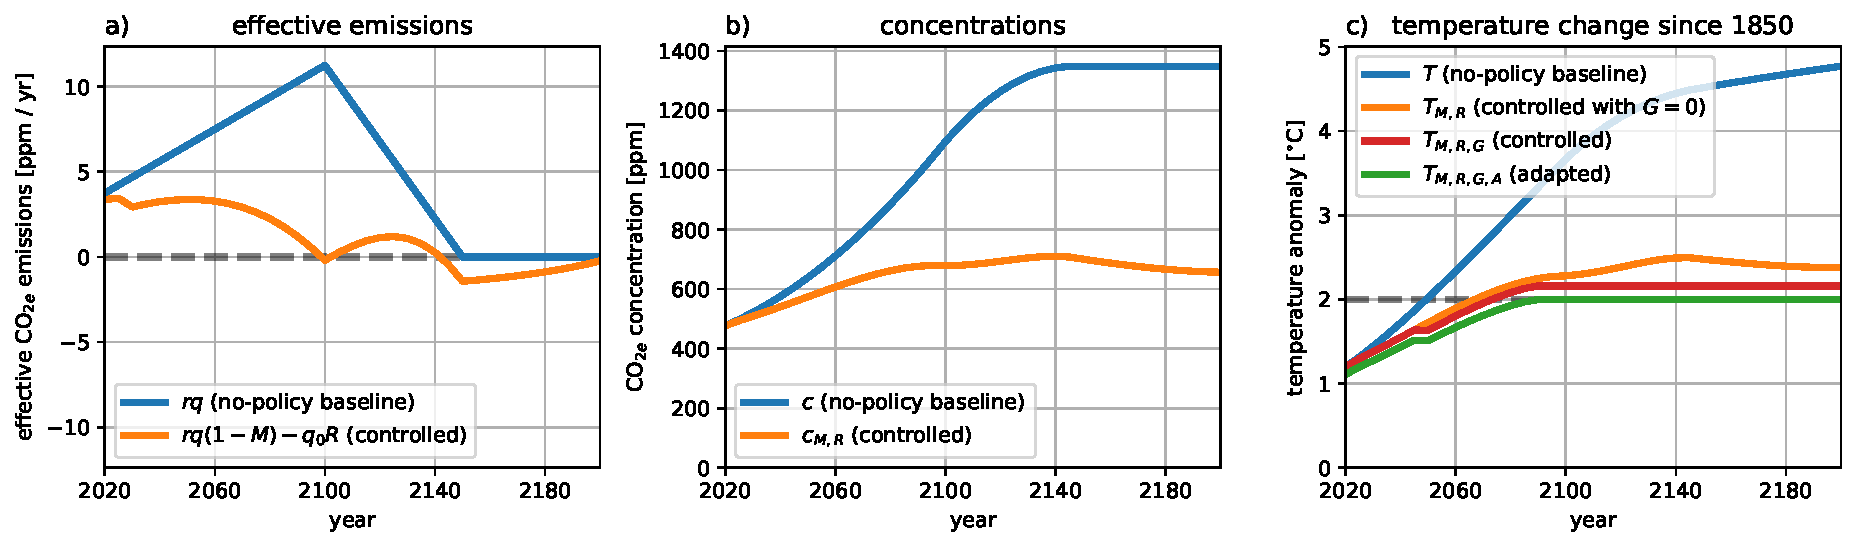
\includegraphics[width=17.8cm]{figures/default-temp_carbon_and_temperatures.pdf}
\caption{Baseline (blue) and optimally-controlled (orange) a) effective CO$_{2e}$ emissions, b) CO$_{2e}$ concentrations, and c) temperature anomaly relative to preindustrial from cost-effectiveness analysis (see Section \ref{sec:cost-effectivness}). Panel c) shows the optimal temperature change that would occur: in a baseline scenario (blue); with just emissions \textbf{M}itigation and carbon dioxide \textbf{R}emoval (orange); with \textbf{M}itigation, \textbf{R}emoval, and solar-\textbf{G}eoengineering (red); and as an ``adapted temperature" (eq. \ref{eq:adapted-temperature}) with \textbf{A}daptation measures also taken into account. The dashed grey line marks the threshold adapted temperature of $T^{\star} = \SI{2}{\celsius}$ to be avoided.}
\label{fig:carbon_and_temperature}
\end{figure*}

\textbf{M}itigation reduces emissions by a factor $M(t) \in [0,1]$ such that the controlled emissions that remain in the atmosphere are $rq(t)\,(1-M(t))$, where $M = 1$ corresponds to complete decarbonization of the economy.

\textbf{R}emoval of CO$_{2e}$, $R(t) \in [0,1]$, in contrast to mitigation, is de-coupled from instantaneous emissions and is expressed as the fraction of 2020 baseline emissions that are removed from the atmosphere in a given year, $q_{0}R(t)$. A maximal value of $R=1$ corresponds to removing $\SI{59}{GtCO_{2e} / year}$, which is more than twice a median estimate of the global potential for negative emission technologies \cite{fuss_negative_2018}.

A useful diagnostic quantity is the effective emissions
\begin{equation}
    rq(t)(1-M(t)) - q_{0}R,
    \label{eq:effective-emissions}
\end{equation} which is the annual rate of CO$_{2e}$ accumulation in the atmosphere (Figure \ref{fig:carbon_and_temperature}a) and is controlled by both mitigation and carbon dioxide removal.
The change in CO$_{2e}$ concentrations is simply the integral of the effective emissions over time (Figure \ref{fig:carbon_and_temperature}b),
\begin{equation}
    c_{M,R}(t) = c_{0} + \int_{t_{0}}^{t} rq(t')(1-M(t')) \text{ d}t' - q_{0} \int_{t_{0}}^{t} R(t')\text{ d}t'.
\end{equation}

\textbf{G}eoengineering by solar radiation management, $G(t) \in [0,1]$, acts to offset a fraction of the CO$_{2e}$ forcing, 
\begin{equation}
    F_{M,R,G}(t) = F_{M,R}(t) - G(t) F(t \rightarrow \infty),
\end{equation}
where $F_{M,R} = a \ln(c_{M,R}(t) / c_{0})$ is the controlled CO$_{2e}$ forcing and $F(t \rightarrow \infty) = \SI{8.5}{W/m^{2}}$ is the maximum baseline CO$_{2e}$ forcing, which is attained starting in 2150. A value of $G = 1$ thus corresponds to a complete cancellation between the baseline equilibrium warming from CO$_{2e}$ and the cooling from reflected solar radiation.

The controlled near-surface air temperature (Figure \ref{fig:carbon_and_temperature}c) evolves according to the total controlled forcing,
\begin{equation}
    T_{M,R,G}(t) - T_{0} = \frac{F_{M,R,G}(t)}{B + \kappa} + \frac{\kappa}{B} \int_{t_{0}}^{t} \frac{e^{\frac{t'-t}{\tau_{D}}}}{\tau_{D}} \frac{F_{M,R,G}(t')}{B+\kappa} \, \text{d}t',
    \label{eq:temperature}
\end{equation}
where $T_{0} = \SI{1.1}{\celsius}$ is the present warming relative to preindustrial and $\tau_{D} = \SI{240}{years}$ is the slow timescale of ocean heat uptake. The first term on the right-hand side of [\ref{eq:temperature}] represents a fast transient response while the second term represents a slow recalcitrant response due to the thermal inertia of the deep ocean. Climate inertia decouples the temperature response from instantaneous forcing and implies that an additional fraction of short-term warming (or cooling) is locked in for the future, even if radiative forcing is stabilized \citep{lickley_time_2019}, as in the case of bringing emissions to zero in our model\footnote{In earth system models with a dynamic carbon cycle, the slow recalcitrant warming due to a reduction in ocean heat uptake happens to be roughly offset by the ocean carbon sink \cite{solomon_irreversible_2009}, such that bringing emissions to zero roughly stabilizes temperatures \citep{matthews_stabilizing_2008}}.

\textbf{A}daptation to climate impacts acts to reduce damages by a fraction $A(t) \in [0, 1/2]$. Since some climate impacts are likely impossible to adapt to \cite[][]{dow_limits_2013}, we assume that adaptation can at most reduce climate damages by one-third. The controlled damages are thus given by
\begin{equation}
    D_{M,R,G,A} = \beta (T_{M,R,G})^{2} (1-A(t)),
    \label{eq:damages}
\end{equation}
where the damage parameter $\beta$ is tuned such that a warming of $\SI{3}{\celsius}$ results in damages of the $2\%$ of Global World Product (GWP). Although adaptation does not affect the planetary temperature directly, it is useful to consider an "adapted temperature" $T_{M,R,G,A}$ which yields controlled damages equivalent to the fully-controlled damages $\beta (T_{M,R,G,A})^{2} = \beta (T_{M,R,G})^{2} (1-A)$ and is defined
\begin{equation}
    T_{M,R,G,A} \equiv T_{M,R,G} \sqrt{(1-A)}.\label{eq:adapted-temperature}
\end{equation}

\subsection*{Costs and benefits of controlling the climate}

The costs of deploying climate controls are non-negligible and must in some way be balanced with the benefits of controlling to climate to avoid damages. The costs of climate controls are parameterized as:
\begin{equation}
    \mathcal{C} = \mathcal{C}_{M} M^{2} + \mathcal{C}_{R} R^{2} + \mathcal{C}_{G} G^{2} + \mathcal{C}_{A} A^{2},
\end{equation}
where the $C_{*}$ are the hypothetical annual costs of fully deploying that control, the values of which are justified in the Methods.

The benefits of deploying climate controls are the avoided climate damages relative to the no-policy baseline scenario,
\begin{equation}
    \mathcal{B} = D - D_{M,R,G,A} = \beta (T^{2} - (T_{M,R,G,A})^{2}).
\end{equation}

\subsection*{Exogenous economic growth}
In contrast to conventional Integrated Assessment Models, which follow classic economic theories of optimal economic growth and solve for the maximal welfare based on the discounted utility of consumption, we here treat economic growth as exogenous. The economy $E(t) = E_{0}(1 + \gamma)^{(t-t_{0})}$ grows from its present value of $E_{0} = \SI{100}{\,trillion\, USD}$ with a fixed growth rate $\gamma = 2\%$, which approximates the economic growth in various simulations of DICE2013r \cite{nordhaus2013dice}. We ignore feedbacks of climate abatement costs and climate damages on economic growth, since they are small variations relative to the exponential rate of economic growth in conventional Integrated Assessment Models \cite{nordhaus2013dice}.

\section*{Optimal deployments of climate controls}\label{sec:optimal-deployment}

If a trusted climate policy decision-maker specifies an objective function to maximize and, optionally, additional policy constraints, the MARGO model is readily optimized in terms of the time-dependent climate control variables $M(t), R(t), G(t), A(t)$. The numerical implementation of the optimization, as well as additional constraints on the permitted timing and rates of deployments which parameterize social, economic, and technological inertia, are described in the Methods. Here, we describe the optimally-controlled results of two policy approaches, cost-benefit analysis and cost-effectiveness analysis, and explore their sensitivity to the discount rate $\rho$ and possible limits to the fractional penetration of mitigation $\mu$, respectively.

\subsection*{Cost-benefit analysis}\label{sec:cost-benefit}

A natural and widely-used objective function is the cost-benefit framework, in which the cost $\mathcal{C}_{M, R, G, A}$ of deploying climate controls is balanced against the benefits $\mathcal{B}_{M, R, G, A}$ of the avoided climate damages. Formally, we aim to maximize the net present benefits:
\begin{gather}
    \max \left\{ \int_{t_{0}}^{t_{f}} 
    \left(\mathcal{B}_{M, R, G, A} - \mathcal{C}_{M, R, G, A} \right) (1 + \rho)^{-(t-t_{0})} \, \text{d}t \right\},
    \label{eq:net-present-benefits}
\end{gather}
where $\rho$ is a discount rate that determines the annual depreciation of future costs and benefits. There are different views about the appropriate non-zero discount rate to apply to multi-generational social utility \cite{ramsey_mathematical_1928, solow_economics_1974, stern_economics_2007}. Here, we choose a discount rate of $\rho = 1\%$, on the low end of values used in the literature, motivated by our preference towards inter-generational equity\footnote{Follow \cite{stern_economics_2007}'s discussion of the discount rate...}.

The results of maximizing net benefits are shown in Figure \ref{fig:cost-benefit}. Early and aggressive emissions mitigation– and to a lesser extent carbon dioxide removal (Fig \ref{fig:cost-benefit}a)– carry net costs of up to 1 trillion USD/year before 2050 relative to the no-policy baseline but deliver orders of magnitude more in benefits from 2050 to 2200 (Fig \ref{fig:cost-benefit}b). Deployments of adaptation and solar-geoengineering are relatively modest, reflecting their relative high costs and the fact that they are further down the causal chain of climate damages and do not directly affect the root cause of the damage: increasing CO$_{2e}$ concentrations due to positive effective emissions.

The preference for controls earlier in the causal chain, notably mitigation, is largely a result of our subjective choice $\rho = 1\%$ for the discount rate. In particular, as the discount rate increases above the economic growth rate, $\rho > \gamma = 2\%$, the decay of the discount factor out-competes economic growth and leads to a different regime of control preferences: the short-term fix offered by solar geo-engineering becomes the dominant control since the high future costs of its unintended climate damages are effectively annulled by the aggressive discounting.

\begin{figure*}%[tbhp]
\centering
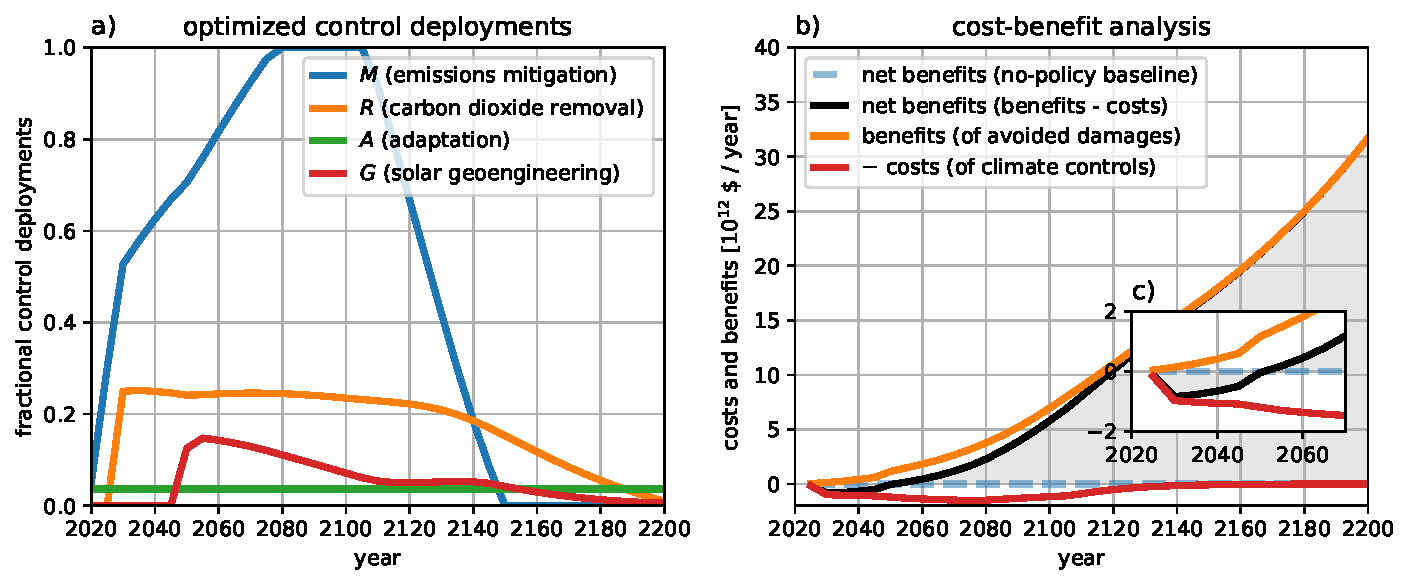
\includegraphics[width=17.8cm]{figures/default-benefits_controls_and_benefits.pdf}
\caption{Results of cost-benefit analysis and sensitivity to the discount rate $\rho$. (a) Optimal control deployments and (b) corresponding discounted costs and benefits relative to the no climate-policy baseline scenario. The total positive area shaded in grey in (b) is the maximal net present benefits (eq. \ref{eq:net-present-benefits}). An inset zooms in on the 2020 to 2050 period of modest net costs. (c) Time-mean control deployments as a function of the discount rate.}
\label{fig:cost-benefit}
\end{figure*}

\subsection*{Cost-effectiveness of avoiding damage thresholds}\label{sec:cost-effectivness}

The conventional cost-benefit approach to understanding climate change is limited by the poorly constrained damage function, which has historically been under-estimated \cite{} and must be continually revised as we understand more about climate surprises lurking at high levels of forcing \citep{alley_abrupt_2003, sherwood_adaptability_2010, scher_carbonocean_2017}. An alternative approach, which presently guides global climate policy negotiations, is to prescribe a threshold of climate damages– or temperatures, as in the Paris Climate Agreement \cite{ParisAgreement2015} - which is not to be surpassed.

In our implementation of the cost-effectiveness approach, we aim to find the lowest net present costs of control deployments
\begin{equation}
    \min\left\{\int_{t_{0}}^{t_{f}} \mathcal{C}_{M,R,G,A} (1 + \rho)^{-(t-t_{0})} \text{ d}t\right\}
    \label{eq:net-present-costs}
\end{equation}
which keep controlled damages below the level corresponding to a chosen temperature threshold,
$\beta (T_{M,R,G})^{2} (1 - A(t)) < \beta (T^{\star})^{2}$, which we rewrite
\begin{equation}
    T_{M,R,G,A} < T^{\star},
\end{equation}
where $T_{M,R,G,A}$ is the "adapted temperature" (eq. \ref{eq:adapted-temperature}) and the threshold $T^{\star} = \SI{2}{\celsius}$ is inspired by the Paris Climate Agreement.

The results of optimizing the cost-effectiveness of controls that keep adapted temperatures below $T^{\star} = \SI{2}{\celsius}$ are shown in Figures \ref{fig:carbon_and_temperature} and \ref{fig:cost-effectiveness}. Fractional emissions mitigation increases proportional to the increase in baseline emissions, reaching $M=\SI{90}{\%}$ decarbonization by 2100, while carbon dioxide is removed at a roughly constant rate of $R q_{0} \approx 20\%\, q_{0} = \SI{1.5}{ppm/year}$ starting in 2030. Since the optimally-controlled temperatures that result from the above cost-benefit analysis are already lower than $T^{\star}$, the optimal controls from cost-effectiveness are less ambitious than for the cost-benefit analysis (Figures \ref{fig:cost-benefit}a, \ref{fig:cost-effectiveness}a). As a consequence of relatively relaxed mitigation and carbon dioxide removal early on, small but non-negligible deployment of solar-geoengineering is used to shave off a few tenths of a degree of warming during its peak in the mid-22nd Century in order to meet the temperature goal (Figure \ref{fig:cost-effectiveness}a and Figure \ref{fig:carbon_and_temperature}c). Adaptation offsets $A = \SI{15}{\%}$ of damages and plays a moderate role in reducing damages below the threshold. Even after discounting, annual costs of control deployments peak in 2100, driven by a peak in mitigation, which is most cost-efficient in 2100 where the baseline emissions are the highest (Figure \ref{fig:cost-effectiveness}b).

To explore the sensitivity of these results to our assumed mitigation costs $\mathcal{C}_{M} M^{2}$, which allow for up to $90\%$ mitigation in 2100 at the relatively low cost of $\SI{1.6}{\;trillion\; USD/year}$, we compare the results against a re-optimization with steeper costs at high levels of mitigation
\begin{equation}
    C_{M}M^{2} \left( 1 - e^{-\left(\frac{1-M}{1-\mu}\right)} \right)^{-1},
    \label{eq:high-mitigation-costs}
\end{equation}
where we set the penetration limit of cheap mitigation to $\mu = 50\%$ and the function's structure is shown in Figure \ref{fig:cost-effectiveness}d. Mitigation costs are unchanged for $M \ll \mu$. Around $M \approx \mu$, low-hanging mitigation options are exhausted and costs begin to increase much more rapidly than the default assumption $M^{2}$. The high costs of deep decarbonization drive a reduction in the peak mitigation from $M=90\%$ to $M=65\%$ in 2100, with some of the reduction being compensated by a more aggressive ramping up of mitigation between 2020 and 2060 (Figure \ref{fig:cost-effectiveness}c). The remainder of the reduced peak mitigation is made up for by a doubling of carbon dioxide removal from $R=20\%$ to $R=40\%$ and an increase in geo-engineering from negligible levels to $G=15\%$ in from 2050 to 2100.


\begin{SCfigure*}%[tbhp]
\centering
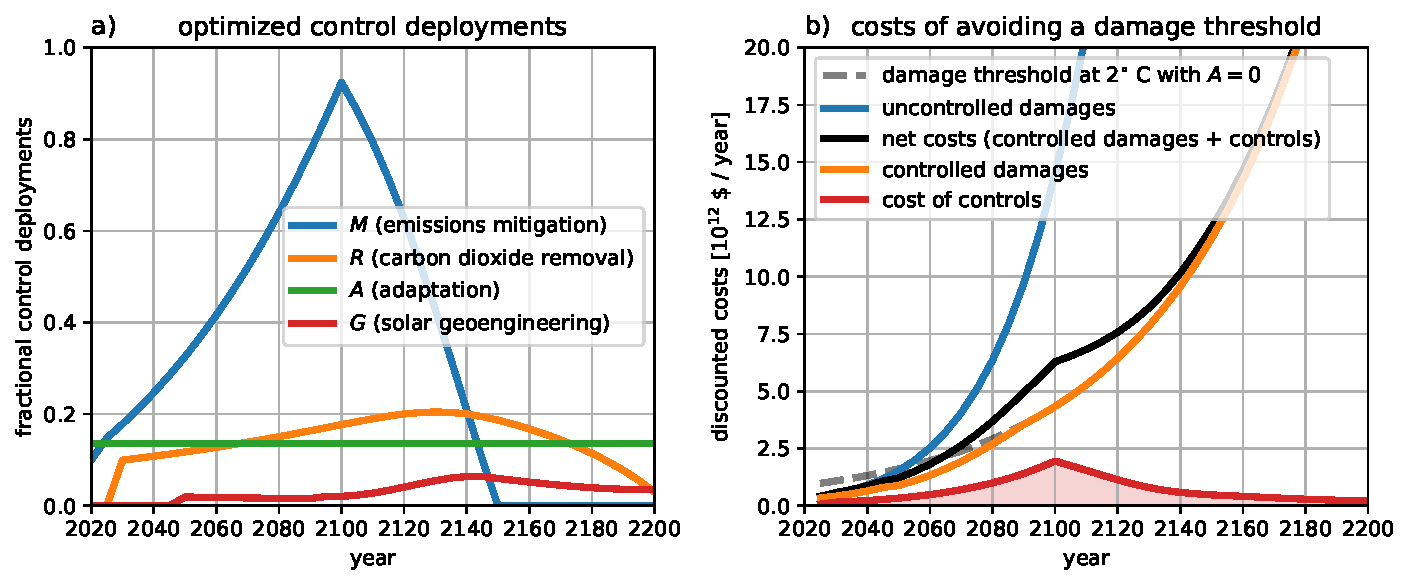
\includegraphics[width=11.4cm]{figures/default-temp_controls_and_damages.pdf}
\caption{Results of cost-benefit analysis and sensitivity to potential limits $\mu$ to mitigation. (a) Optimal control deployments and (b) corresponding costs and damages. In panel (b), the blue line shows the discounted baseline uncontrolled damages; the dashed grey line shows the discounted damages associated with $2^{\circ}$ of warming, which are to be avoided at all costs; the orange line shows the discounted damages in the optimally-controlled solution; and the red line shows the optimal discounted costs of controls such that the shaded area below is the minimal net present costs of controls (eq. \ref{eq:net-present-costs}). (c) Control deployments, as in (a), but re-optimized with high costs of deep decarbonization (blue line in d, eq. \ref{eq:high-mitigation-costs}) relative to the default mitigation costs (black line in d). Mitigation in the default scenario (a) is reproduced as a dashed line in (c) for ease of comparison.}
\label{fig:cost-effectiveness}
\end{SCfigure*}

\section*{A policy process for responding to uncertain future outcomes}

Integrated Assessment Modelling (IAM) approaches assume perfect foreknowledge of model dynamics, parameters (or parameter distributions), and inputs. Future outcomes will differ from projections because the models are imperfect approximations of the socio-economic and physical climate systems they represent. For example, socio-economic models may assume erroneous future costs of climate controls and physical climate models may omit tipping elements \citep{steffen_trajectories_2018}, both of which would lead to biases in model projections with respect to actual outcomes. Furthermore, the assumption of perfect foreknowledge degrades the active roles of policy decision-makers in determining baselines and control cost functions and of climate researchers in refining estimates of physical model parameters.

A hypothetical trusted climate policy decision-maker must be in a position to respond to the inevitable differences that arise between model projections and actual outcomes and to revise their system understanding based on the newest developments in research. We show how our model equips climate policy decision-makers with the ability to periodically re-evaluate policy prescriptions by revising the underlying model structure and parameter values to correct for revealed biases.

The responsive control strategy process we propose is as follows:
\begin{enumerate}
    \item Initial future trajectories of optimal control deployments are computed from the vantage point of $t=t_{0}$;
    \item Model projections and control deployments are integrated forward one policy-making period to $t_{1}=t_{0} + \Delta t$;
    \item Model structure and parameter values are revised, owing to new information;
    \item Future trajectories of control deployments are re-optimized, now from the vantage point of $t_{1}=t_{0}+\Delta t$ and with revised model parameters;
    \item Return to step 2, replacing $t_{1} = t_{0} + \Delta t$ with $t_{n} = t_{n-1}+\Delta t$ for period $n$, and repeat the process for the desired number of periods.
\end{enumerate}

To illustrate the utility of the policy response process, we apply it to three hypothetical future scenarios, in which the most cost-effective controls for keeping adapted temperatures below $T^{\star} = \SI{2}{\celsius}$ are sequentially re-optimized in response to changes in model inputs and parameters.

\begin{SCfigure*}%[tbhp]
\centering
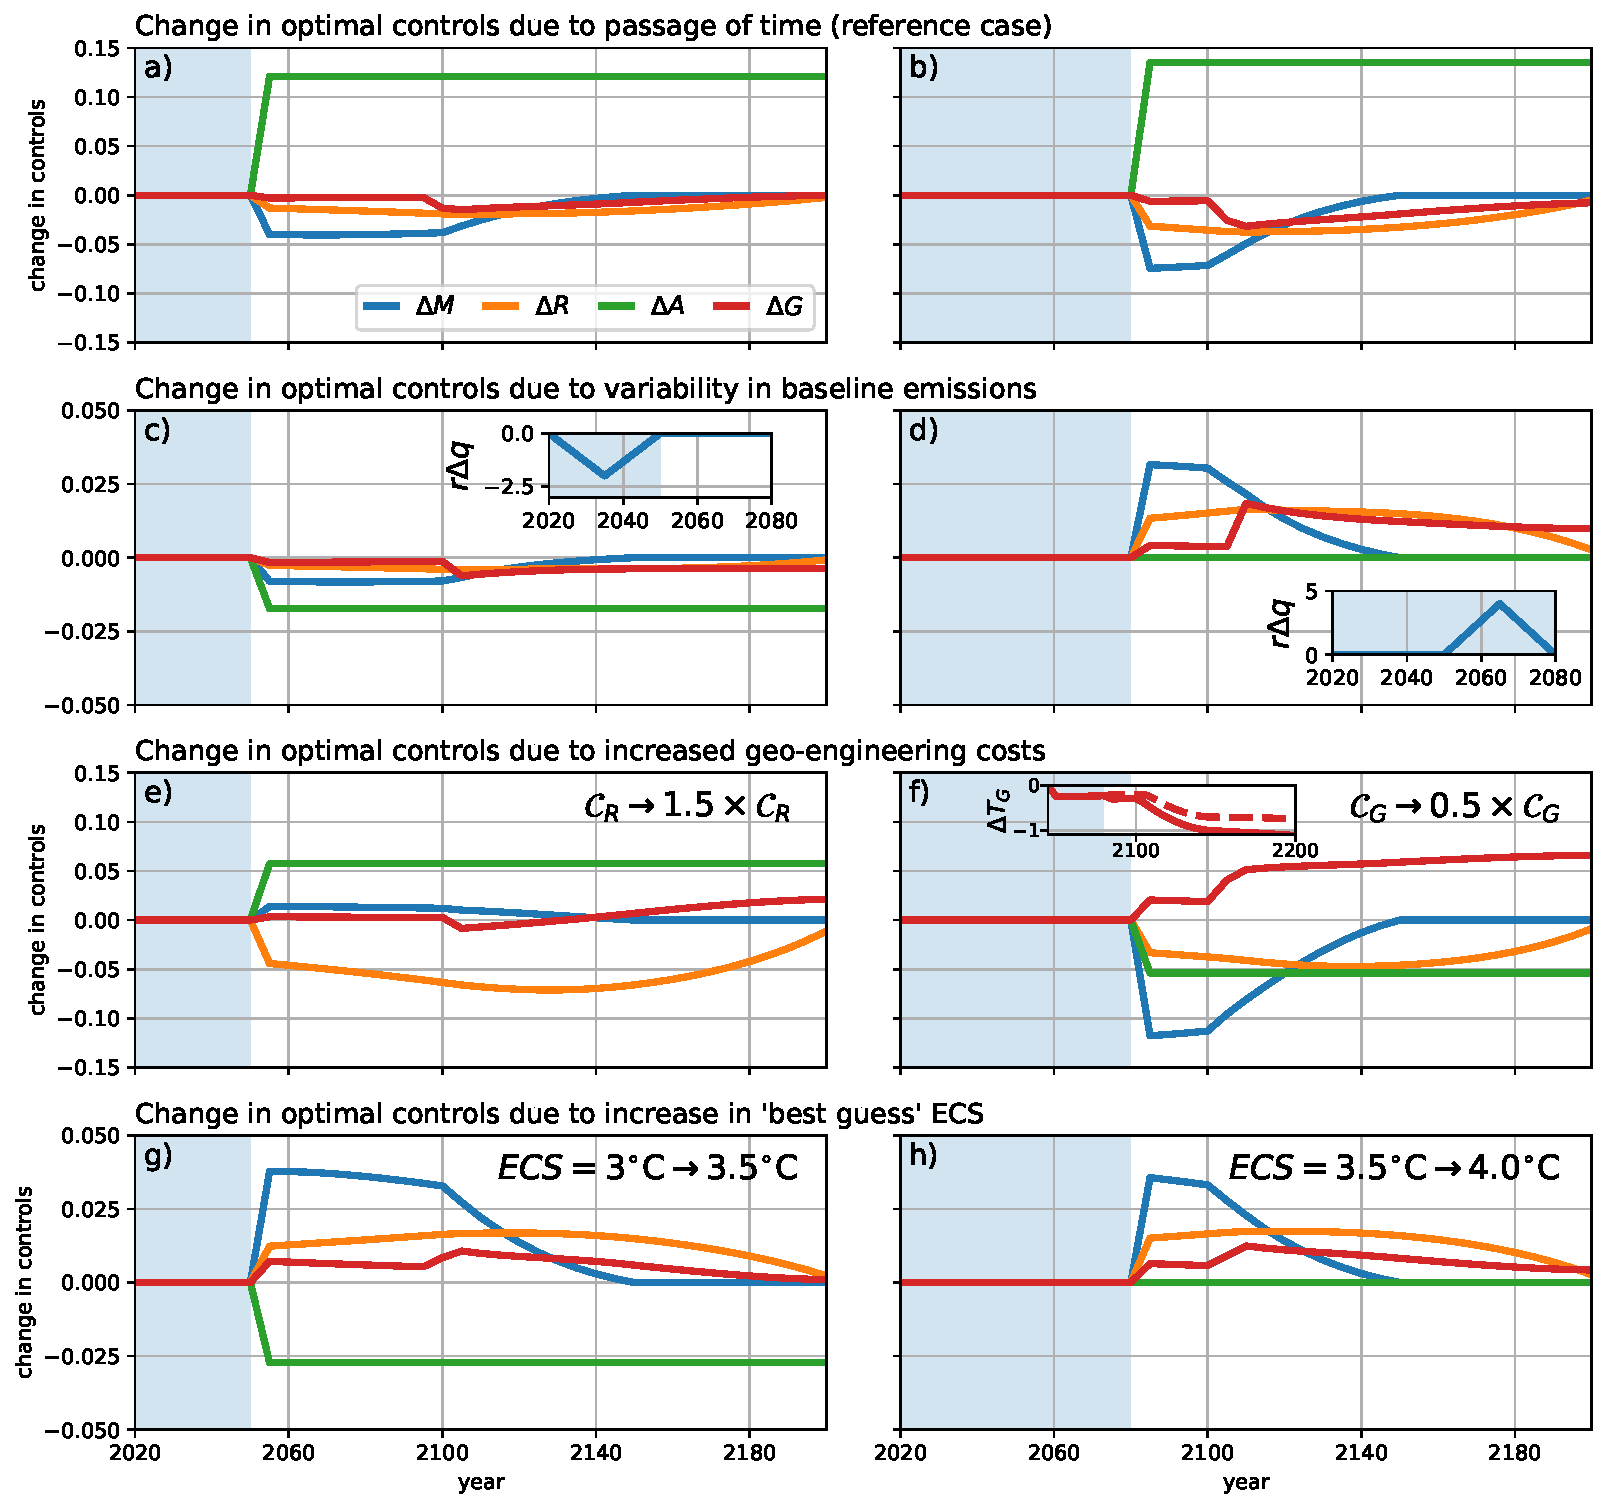
\includegraphics[width=11.4cm]{figures/policy_updates.pdf}
\caption{Illustration of a proposed responsive policy progress. (a-f) Changes in the optimally cost-effective control trajectories at keeping adapted temperatures below the threshold $T^{\star} = \SI{2}{\celsius}$, relative to those shown in Figure \ref{fig:cost-effectiveness}a for the default model parameters. The changes in control deployments shown here are due to sequential re-optimization at 2050 and 2080 with revised model parameters: (c,d) where historical effective emissions $rq(t)$ are sequentially decreased and then increased (see insets); (e,f) where the costs of carbon and solar geo-engineering are sequentially increased and decreased, respectively; and (g,h) where the best guess of the Equilibrium Climate Sensitivity (ECS) is revised upwards in 2050 and again in 2080. The inset in (d) shows the cooling due to solar geo-engineering $\Delta T_{G} = T_{M,R,G} - T_{M,R}$ in the default scenario (dashed) and after the re-evaluation in 2080 shown in panel (d) (solid).}
\label{fig:policy-updates}
\end{SCfigure*}

\subsection*{Scenario 1: revealed bias in projected near-term baseline emissions}

Suppose in $t_{0} = 2020$ that the trusted policy decision-maker prescribes aggressive climate control policies based on their cost-effectiveness at keeping warming below $T^{\star} = \SI{2}{\celsius}$ (step 1; Figure \ref{fig:cost-effectiveness}a) and these optimal climate controls are perfectly implemented over the following $\Delta t = 30$ years (step 2).

The policy decision-maker directs a re-evaluation of the optimal control strategy at $t_{1} = 2050$. The actual baseline emission trajectory between $t_{0}=2020$ and $t_{1}=2050$ is found to be $r\Delta q = \SI{1}{ppm/year}$ lower than projected on average (Figure \ref{fig:policy-updates}a, inset), resulting in lower CO$_{2e}$ concentrations than anticipated and projected maximum warming of $T_{M,R,G,A} = \SI{1.9}{\celsius}$, well below the $T^{\star} = \SI{2}{\celsius}$ goal. The model inputs are thus revised to account for these lower-than-expected historical baseline emissions (step 3) and the optimal future control trajectories are re-computed (step 4). This would imply a larger remaining carbon budget \citep{millar_cumulative_2016} and allows the policy decision-maker to relax control deployments while still remaining below $T^{\star} = \SI{2}{\celsius}$ of warming (Figure \ref{fig:policy-updates}a), resulting in $6$ trillion USD of avoided net present costs of control deployments. At this point, the policy decision maker must decide whether to continue existing policies that lead to less than $\SI{1.9}{\celsius}$ of warming or to reduce future controls deployments (and costs) at the risk of an additional $\SI{0.1}{\celsius}$ of warming.

Suppose that, after following the re-optimized control trajectories for another $\Delta t = \SI{30}{years}$ (step 5), the historical effective baseline emissions must now be revised upwards by $\SI{2}{ppm/year}$ on average (Figure \ref{fig:policy-updates}b, inset). With existing policies, the increased historical emissions would result in a $\SI{0.15}{\celsius}$ overshoot of the $T^{\star} = \SI{2}{\celsius}$ degree goal. The most cost-effective adjustment to existing control policies that is consistent with the temperature goal is to increase mitigation efforts by an additional $\Delta M = 5\%$ (Figure \ref{fig:policy-updates}b), at a net-present cost of $6$ trillion USD.

\subsection*{Scenario 2: revealed bias in projected geoengineering costs}

Suppose that at a re-evaluation in 2050, carbon dioxide removal is $\SI{50}{\%}$ more expensive than projected. The climate policy-maker directs deployment of the most cost-effective control trajectories which keep warming below $T^{\star}=\SI{2}{\celsius}$, which are re-optimized with the revised cost of carbon dioxide removal. The result is to decrease carbon dioxide removal by $\Delta R = \SI{-5}{\%}$, increase adaptation by $\Delta A = 5\%$, and increase mitigation by $\Delta M = \SI{3}{\%}$ (Figure \ref{fig:policy-updates}c). The shift away from expensive carbon dioxide removal towards cheaper mitigation and adaptation results in $3.5$ trillion USD of avoided net present costs of control deployments, with little difference in climate damage outcomes.

Suppose that after an additional \SI{30}{years}, during which solar geoenengineering is ramped up to a modest but non-zero level $G=\SI{5}{\%}$ (Figure \ref{fig:cost-effectiveness}a), it becomes clear that the costs of unintended side-effect damages of solar geoengineering are less than half as large as expected. In this scenario, the optimal future trajectory is to expand solar-geoengineering deployments in the 22nd Century to $G \approx \SI{10}{\%}$ (resulting in $\Delta T_{G} = T_{M,R,G} - T_{M,R} \approx \SI{-0.5}{\celsius}$ of cooling, up from $\SI{-0.25}{\celsius}$; Figure \ref{fig:policy-updates}d, inset) and reduce peak mitigation levels by $\Delta M = \SI{-10}{\%}$ (Figure \ref{fig:policy-updates}d), resulting in $3.8$ trillion USD of avoided net present costs.

\subsection*{Scenario 3: revealed bias in estimates of climate sensitivity}

Suppose that by 2050, a dramatically improved suite of general circulation climate models robustly exhibits Equilibrium Climate Sensitivities of $ECS=\SI{3.5}{\celsius}$, up from $\SI{3}{\celsius}$ in recent years \citep{geoffroy_transient_2012}, and further improvements result in $ECS=\SI{4}{\celsius}$ by 2080. Each of these revisions effectively shrinks the remaining cumulative carbon budget and thus require sequentially increased deployments of mitigation in order to keep warming below $T^{\star} = \SI{2}{\celsius}$ (Figures \ref{fig:policy-updates}g, h). This responsive policy process only works if adjustments are made sufficiently frequently: if the policy decision-maker had waited $2\Delta t = 60$ years before re-evaluating their course, with $ECS=\SI{4}{\celsius}$ there would already be enough warming baked into the system that $T^{\star} = \SI{2}{\celsius}$ would be inevitable; at best, temperatures could be kept below $\SI{2.1}{\celsius}$.

This section demonstrates it is possible to define a policy response process that permits a climate policy decision-maker to make successive adjustments to climate control strategies based on evolving outcomes and research developments. A disciplined response process thus simultaneously reaps the benefits of early action and minimizes the potential for regret by periodically adjusting for revealed policy or model deficiencies.

\section*{Discussion}



Here, we only price damages due to temperature changes (via the climate damage function, eq. \ref{eq:damages}) and CO$_{2e}$ forcing (via solar geo-engineering costs), which are further down the causal chain of climate damages than CO$_{2e}$ emissions and concentrations, which carry their own indepedent costs: increased CO$_{2e}$ concentrations drive ocean acidification and CO$_{2e}$ emissions are tied to air pollution \cite{silva_global_2013, burnett_global_2018}. Including these co-benefits of abatement, which occur earlier in the causal chain of climate damages, would act to favor emissions mitigation over other controls as it is the only control to address the problem directly at its source.

The greatest caveat of the present study is the assumption of a single trusted decision-maker. The costs and benefits defined here are globally-aggregated; assymetric costs and benefits between different regions introduces the "free-rider" for abatement and R\&D and the "free-driver" problem for solar-geoengineering deployment. The interactions between these effects can be counter-intuitive: \cite{moreno-cruz_mitigation_2015} find that high asymmetry in solar geo-engineering damages drives high levels of mitigation so that "free-driver" solar geo-engineering is avoided at all costs. Further issues arise if the decision-maker's motives are unknown or the implementation of their policies are sub-optimal.

\matmethods{
All data used in the study can be found at \url{github.com/hdrake/OptimizeClimate} or can be reproduced by the Jupyter notebooks therein.

\subsection*{Two-box energy balance model}

The evolution of the global-mean near-surface temperature anomaly (relative to the initial time $t_{0} = 2020$) is determined by the two-box linear energy balance model \citep[e.g][]{gregory_vertical_2000, held_probing_2010}:
\begin{gather}
    C_{U} \dv{T}{t} = -B T - \kappa( T - T_{D}) + F(t), \label{eq.upper_ocean}
    \\
    C_{D} \dv{T_{D}}{t} = \kappa (T - T_{D}),\label{eq.deep_ocean}
\end{gather}
where eq. \ref{eq.upper_ocean} represents the upper ocean with average temperature anomaly $T$, and eq. \ref{eq.deep_ocean} represents the deep ocean with an average temperature $T_{D}$. The near-surface atmosphere exchanges heat rapidly with the upper ocean and thus the global-mean near-surface air temperature is also given by $T$. The physical model parameters are: the upper ocean heat capacity $C_{U} = \SI{7.3}{W\; yr\; m^{-2}\; K^{-1}}$ (including a negligible contribution $C_{A} \ll C_{U}$ from the atmosphere); the deep ocean heat capacity $C_{D} = \SI{106}{W\; yr\; m^{-2}\; K^{-1}}$; the climate feedback parameter $B = \SI{1.13}{W\; m^{-2}\; K^{-1}}$; and the ocean mixing rate $\kappa = \SI{0.73}{W\; m^{-2}\; K^{-1}}$. The parameter values are taken from the multi-model mean of values diagnosed from 16 CMIP5 models \cite{geoffroy_transient_2012}. The radiative forcing and temperature anomalies at $t_{0} = 2020$ relative to preindustrial are $F(t_{0}) - F(t_{\text{pre}}) = \SI{2.5}{W\, m^{-2}}$ and $T_{0} \equiv T(t_{0}) - T(t_{\text{pre}}) = \SI{1.1}{K}$, where we set $F_{0} \equiv F(t_{0}) = \SI{0}{W\, m^{-2}}$ and $T(t_{\text{pre}}) = \SI{0}{K}$ for convenience.

Since, by construction, the anthropogenic forcing $F(t)$ varies on timescales longer than the fast relaxation timescale $\tau_{U} = C_{U}/(B + \kappa) = \SI{4}{years}$, we can ignore the time-dependence in the upper ocean and approximate
\begin{equation}
    T \approx \frac{F+\kappa T_{D}}{B + \kappa},
    \label{eq.shallow_approx}
\end{equation}
where the evolution of the deep ocean
\begin{equation}
    C_{D} \dv{T_{D}}{t} \approx - \frac{B \kappa}{B + \kappa} T_{D} + \frac{\kappa}{B + \kappa} F
    \label{eq.deep_ode}
\end{equation}
occurs on a slower timescale $\tau_{D} \equiv \dfrac{C_{D}}{B} \dfrac{B + \kappa}{\kappa} = \SI{240}{years}$ \citep{held_probing_2010}. This approximation is convenient because it permits a simple closed form solution, but should be avoided if the model is applied to scenarios with rapidly changing forcing, such as studies of the transient response to an instantaneous doubling of CO$_{2}$ or the solar geo-engineering "termination effect". Plugging the exact solution to eq. \ref{eq.deep_ode} into eq. \ref{eq.shallow_approx} gives the closed-form solution
\begin{equation}
    T(t) - T_{0} = \frac{F(t)}{B + \kappa} + \frac{\kappa}{B} \frac{1}{(B+\kappa)} \int_{t_{0}}^{t} \frac{ e^{-(t-t')/\tau_{D}}}{\tau_{D}} F(t') \, \text{d}t'.\label{eq:baseline_temperature}
\end{equation}
The evolution of the controlled temperature anomaly (eq. \ref{eq:temperature}; Figure \ref{fig:carbon_and_temperature}c) has the same form but is instead driven by the controlled net radiative forcing $F_{M,R,G}$.

We identify the first term on the right hand side of eq. \ref{eq:baseline_temperature} and eq. \ref{eq:temperature} as the transient climate response \citep{gregory_transient_2008}, which dominates for $t-t_{0} \ll \tau_{D}$, while the second term is a slower ``recalcitrant" response due to a weakening of ocean heat uptake as the deep ocean comes to equilibrium with the upper ocean \citep{held_probing_2010}. While the contribution of the recalcitrant component to historical warming is thought to be small, it contributes significantly to 21st century and future warming \citep{gregory_transient_2008,held_probing_2010}.

The behavior of the model on short and long timescales is illustrated by applying it to the canonical climate change experiment in which CO$_{2}$ concentrations increase at 1\% per year until doubling. The temperature anomaly first rapidly increases until it reaches the Transient Climate Sensitivity $TCS = \dfrac{F_{2\times}}{B + \kappa} = \SI{1.9}{\celsius}$ around the time of doubling $t=t_{2\times}$, with $t_{2\times} - t_{0} \ll \tau_{D}$ and $F_{2\times} = \alpha \ln(2)$, and then gradually asymptotes to the Equilibrium Climate Sensitivity $ECS = \dfrac{F_{2\times}}{B} = \SI{3.1}{\celsius} > TCS$ on a much longer timescale $t-t_{0} \gg \tau_{D}$.

\subsection*{Improved realism of ocean heat uptake relative to DICE}
Despite our temperature projection model having the same functional form as the DICE-2013r model \cite{nordhaus2013dice}, the character of their temperatures projections are dramatically different from ours due to the apparently unphysical calibration of the DICE-2013r model parameters. Their value of the deep ocean uptake parameter $\kappa = \SI{0.088}{W m^{-2} K^{-1}}$ (which they call $\zeta_{3}$) is inexplicably one-fifth of their previous iteration in DICE-2010 \cite{calel_physics_2016} and is almost an order of magnitude smaller than our value $\kappa = \SI{0.73}{W\; m^{-2}\; K^{-1}}$, which is taken from a well-tested calibration to CMIP5 models that is based on climate physics \cite{geoffroy_transient_2012}. DICE-2013r apparently compensates for the essentially non-existent deep ocean heat uptake by increasing the upper-ocean heat capacity by an order of magnitude relative to the \cite{geoffroy_transient_2012} value, which leads to an upper ocean timescale of $\tau_{U} = \SI{36}{years}$ that leads to a much more sluggish climate response than the realistic value of $\tau_{U} = \SI{4}{years}$ used here. In simulated experiments with either rapidly changing forcing ($\Delta t \ll \tau_{U}$) or involving long timescales ($t \gg \tau_{U}$), the current implementation of the DICE energy balance model, which is used in both DICE-2013r \cite{nordhaus2013dice} and DICE-2016 \cite{nordhaus_revisiting_2017}, yields erroneous results (Figure S1 and SI text). When considering multi-centennial scenarios with fast-acting climate controls like solar-geoengineering, both of these conditions apply and one should be wary of analyses that use the DICE model, at least until its ocean heat uptake dynamics are improved \cite{calel_physics_2016}.

\subsection*{Control costs}
The scaling costs for the four controls used in the present study are subjectively chosen, but we here describe our rationale. We remind the reader that the purpose of the model is to reveal insights about trade offs between the multiple controls and the dependence of model results on structural and parameteric choices. The interested reader can choose their own parameter values and see how the results change by visiting our browser application at \url{github.com/hdrake/OptimizeClimate}.

The costs of mitigation are set according to the IPCC WG3 Fifth Assessment Report \cite{}. In aggressive mitigation scenarios where CO$_{2e}$ emissions decrease $78\%$ to $118\%$ by 2100, they estimate abatement costs of about $2\%$ of GWP (see their Figure 6.21). Thus, we set the scaling cost of mitigation controls to $\mathcal{C}_{M} = \tilde{\mathcal{C}}_{M} E(t)$, where the cost of mitigating all emissions is $\tilde{\mathcal{C}}_{M} = 2\%$ of the GWP $E(t)$.

The costs of carbon dioxide removal are set according to bottom-up cost estimates from \cite[][their Table 2]{fuss_negative_2018}. We compute the mean of the median cost for each negative-emissions technology (in USD/tCO$_{2}$), where each technology's cost is weighted by its upper-bound potential (in GtCO$_{2}$/year). This leads to a total potential of roughly $q_{0}/2 \approx \SI{26}{GtCO_{2}/year}$ at an average cost of $\overline{C}_{R}= \SI{110}{USD/tCO_{2}}$. The scaling cost is thus set based on an estimate for $R=50\%$, i.e. $\mathcal{C}_{R} \left(\frac{1}{2} \right)^{2} = \overline{C}_{R}\; q_{0} /2$ or $\mathcal{C}_{R} = 2 \overline{C}_{R}\; q_{0} = 6.4$ trillion USD/year.

The costs of solar-geoengineering largely reflect the costs of unintended climate damages that result due to their imperfect compensation for greenhouse gas forcing \cite{irvine_towards_2017}. Relative to both the costs of unintended damages and the costs of other climate controls, the direct costs of solar geo-engineering measures are thought to be small \citep{mcclellan_cost_2012}, as in the most commonly studied proposal of releasing gaseous sulfate aerosol precursors into the stratosphere to reflect sunlight back to space. The reference cost of geoengineering is thus given by $\mathcal{C}_{G}(t) = \tilde{\mathcal{C}}_{G} E(t)$, where $\tilde{\mathcal{C}}_{G}$ is the damage due to deploying $-F_{\infty} \equiv -F(t \rightarrow \infty) = \SI{-8.5}{W m^{-2}}$ worth of solar radiation management, as a fraction of the exogenous GWP $E(t)$. In the face of considerable uncertainties about the climate impacts of large-scale solar geoengineering \citep{irvine_towards_2017}, we make the conservative assumption that the unintended damages of solar geoengineering are as large as the uncontrolled damages due to an equivalent amount of CO$_{2e}$ forcing \citep[as in][]{goes_economics_2011, belaia_optimal_2019}, i.e. $\tilde{\mathcal{C}}_{G} \equiv \tilde{\beta} (F_{\infty}/B)^{2} \approx \SI{4.6}{\%}$, where $F_{\infty}/B$ is the equilibrium temperature response to a fixed radiative forcing of $F_{\infty} = \SI{8.5}{W m^{-2}}$.

The costs of adaptation are estimated based on a recent joint report from the United Nations, the Bill and Melinda Gates Foundation, and the World Bank. They estimate that adaptation measures costing $1.8$ trillion USD from 2020 to 2030 generate more than five times as much in total net benefits. Here, we make the crude assumption that this level of spending ($180$ billion USD / year) reduces climate damages by $A=20\%$, i.e. $\mathcal{C}_{A} \left( \frac{1}{5} \right)^{2} = 180$ billion USD / year, or $\mathcal{C}_{A} = 4.5$ trillion USD / year. As mentioned above, we additionally cap adaptation at $A<1/2$, recognizing that adaptation to all climate impacts is impossible: there will always be residual damages that can not be adapted to.

\subsection*{Social, technological, and economic inertia}


\subsection*{Optimization method}
We use the Interior Point Optimizer \cite{wachter_implementation_2006} (\url{https://github.com/coin-or/Ipopt}), an open source software package for large-scale nonlinear optimization, to minimize objective functions representing benefits and costs to society subject to assumed policy constraints. In practice, the control variables $\alpha \in \mathcal{A} = \{ M, R, G, A\}$ are discretized into $N = (t_{f} - t_{0}) / \delta t$ timesteps (default $\delta t = \SI{5}{years}$) resulting in a $4N$-dimensional optimization problem. In the default (deterministic and convex) configuration, the model takes only $\mathcal{O}(\SI{10}{ms})$ to solve after just-in-time compiling and effectively provides user feedback in real time.  This makes the model amenable to our forthcoming interactive web application (e.g. following the lead of the impactful En-ROADS model \cite{siegel2018roads}. The model has been designed for use in stochastic simulations where the determinstic scalar objective function can be generalized to an expected value of many simulations and determinstic constraints can be generalized to probablistic constraints, although these features are still in testing.

\subsection*{Model validation} In Section 2 of the Supplementary Information, we show that by tweaking just a few of these default parameter values, the model replicates the qualitative results of studies ranging from analytical control theory analysis of solar-geoengineering deployments \cite{soldatenko_optimal_2018} to numerical optimizations of mitigation, carbon dioxide removal, and solar geo-engineering deployments in a recent application of DICE \cite{belaia_optimal_2019}, a commonly used Integrated Assessment Model \cite{nordhaus_optimal_1992}.
}

\showmatmethods{} % Display the Materials and Methods section

\acknow{}

\showacknow{} % Display the acknowledgments section

% Bibliography
\bibliography{references, refs_by_hand, refs_extra}

\end{document}
